\documentclass[a4paper,10pt]{article}
\usepackage[margin=2cm]{geometry}
\usepackage[thinfonts]{uglix2}
\usepackage{ulem}
\nouveaustyle
\begin{document}
\titre{Contrôle 01}{NSI2}{09/2020}

{\color{UGLiBlue}\Huge\titlefont Partie 1 : sur papier\\}

\exo{ - Fonction d'Ackermann-Péter\hfill 4pts}

Cette fonction est définie pour tout $m\in\N$ et tout $n\in\N$ par
 $$A(m,n)=\begin{cases}
	n+1 & \mbox{si } m=0\\
	A(m-1,1) &\mbox{si } m>0\mbox{ et } n=0\\
	A(m-1,A(m,n-1)) &\mbox{si } m>0\mbox{ et } n>0\\
\end{cases}$$

\'Ecrire la fonction $A$ en \textsc{Python}.\\

\begin{encadre}[Réponse]
On peut recopier tel quel, mais on peut aussi utiliser \pythoninline{if elif else} comme ceci :
\inputminted{python}{scripts/ackermann.py}
\end{encadre}


\exo{ - Fonction mystère\hfill 4pts}

Que fait la fonction suivante ? Ne pas expliquer le code ligne par ligne, dire ce que renvoie la fonction par rapport au paramètre d'entrée.
\pythonfile{scripts/mystery.py}
\begin{enumerate}[\bfseries 1.]
	\item 	Que renvoie \pythoninline{mystery([1])} ?\\
    \begin{encadre}[Réponse]
    \pythoninline{mystery([1])} renvoie \pythoninline{[1]} : c'est un cas d'arrêt.
    \end{encadre}
	\item 	Que renvoie \pythoninline{mystery([1, 2, 3])} ?\\
    \begin{encadre}[Réponse]
    \pythoninline{mystery([1, 2, 3])} renvoie \pythoninline{[3] + mystery([2]) + [1]} ce qui donne \pythoninline{[3, 2, 1]}.
    \end{encadre}
    \item   Quel est le rôle de cette fonction ?\\

\begin{encadre}[Réponse]
Lorsque la liste est vide ou contient un seul élément, la fonction renvoie cette même liste, sinon elle une liste dont le premier élément est le dernier de \pythoninline{lst}, dont le dernier est le premier de \pythoninline{lst} et dont la liste du \og milieu\fg{} est le résultat d'un appel récursif.\\
Pour faire simple, elle permute les extrémités de la liste et fait de même avec la sous-liste composée de cette liste sans les extrémités.\\
Ainsi la fonction renvoie la liste de départ en inversant l'ordre des éléments.
\end{encadre}
\end{enumerate}
\exo{}\\

On veut construire une base de données d'\oe uvres artistiques. Voici un résumé des données que l'on a récoltées :
\begin{center}
\textbf{Œuvre}\\[1em]

\begin{tabular}{|c|c|c|c|c|}
\hline
\rowcolor{UGLiOrange} \textbf{\color{white}id} &\textbf{\color{white}titre}&\textbf{\color{white}creation}&\textbf{\color{white}id\_categorie}&\textbf{\color{white}id\_artiste}\\
\hline
130&Cheval et cavalier &1511 &5 &40\\
196&Colombe de la paix &1949 &2 &56\\
454&Guernica &1937&4&56\\
546&L'Homme de Vitruve&1490&2&40\\
591&L'escalier de Chambord&1516&3&40\\
634&La Cène&1498&4&40\\
649&Les Éléphants&1948&4&78\\
685&La Girafe en feu&1937&4&78\\
706&La Joconde&1519&4&40\\
...&... & ... & ... & ...\\
\hline
\end{tabular}\\[2em]

\textbf{Artiste}\\[1em]

\begin{tabular}{|c|c|c|c|}
\hline
\rowcolor{UGLiOrange} \textbf{\color{white}id} &\textbf{\color{white}nom}&\textbf{\color{white}naissance}&\textbf{\color{white}mort}\\
\hline
40 & Léonard de Vinci & 1452 & 1519\\
56 & Pablo Picasso & 1881 & 1973 \\
78 & Salvador Dali & 1904 & 1989\\
\hline
\end{tabular}\\[2em]

\textbf{Catégorie}\\[1em]

\begin{tabular}{|c|c|}
\hline
\rowcolor{UGLiOrange} \textbf{\color{white}id} &\textbf{\color{white}classement}\\
\hline
1 & céramique \\
2 & dessin \\
3 & objet \\
4 & peinture \\
5 & sculpture \\
\hline
\end{tabular}
\end{center}
Seul le premier tableau n'est pas donné en entier car il comporte trop de lignes.


Donner le modèle relationnel en ligne de la BDD. Ne pas oublier d'indiquer les types des attributs, de souligner en trait plein les clés primaires et en pointillés les clés étrangères.

\begin{encadre}[Réponse]
Voici un modèle possible :

\textbf{Artiste}(\uline{id\_artiste INTEGER}, nom TEXT, naissance DATE, mort DATE)\\

\textbf{Categorie}(\uline{id\_categorie INTEGER, classement TEXT})\\

\textbf{Œuvre}(\uline{id INTEGER}, titre TEXT, creation DATE, \dashuline{id\_categorie}, \dashuline{id\_artiste})
\end{encadre}

\exo{ - CinéHit, c'est plus de hits !\hfill 16pts}


Voici le schéma relationnel de la base de données du site de cinéphiles CinéHit :\\

\begin{encadrecolore}{Schéma relationnel}{UGLiGreen}

\begin{enumerate}[\textbullet]
	\item 	\textbf{Realisateur}(\uline{id\_realisateur INTEGER}, nom VARCHAR(48))\\
	\item 	\scriptsize\textbf{Internaute}(\uline{id\_internaute INTEGER}, prenom VARCHAR(32), nom VARCHAR(32), inscription DATE, email VARCHAR(64))\\\normalsize
            Avec la contrainte utilisateur que l'inscription est postérieure à \texttt{2003-01-01} et que l'email est unique.\\
    \item   \textbf{Genre}(\uline{id\_genre INTEGER}, categorie VARCHAR(24))\\
            Avec la contrainte que la catégorie est unique.\\

     \item  \scriptsize\textbf{Film}(\uline{id\_film INTEGER}, titre VARCHAR(128), sortie DATE, duree INTEGER, \dashuline{genre INTEGER}, \dashuline{realisateur INTEGER}, moyenne DECIMAL)\\\normalsize
     Avec la contrainte que la sortie est postérieure à 1895.\\
     La clé étrangère genre référence la clé primaire id\_genre de la relation \textbf{Genre}, et la clé étrangère realisateur référence la clé primaire id\_realisateur de la relation \textbf{Realisateur}.\\
     L'attribut duree est la durée du film convertie en minutes, et l'attribut moyenne est un nombre décimal entre 0 et 10 et comportant un chiffre après la virgule.\\
     \item \textbf{Note}(\uline{\dashuline{film INTEGER}, \dashuline{internaute INTEGER}}, points INTEGER)\\
     Avec la contrainte que les points sont entre 0 et 10.\\
     La clé primaire est le couple (film, internaute) formé de la clé étrangère film qui référence la clé primaire id\_film de la relation \textbf{Film} et la clé étrangère internaute qui référence la clé id\_internaute  de la relation \textbf{Internaute}.

\end{enumerate}






\end{encadrecolore}
On peut résumer tout ceci par le diagramme ci-dessous.


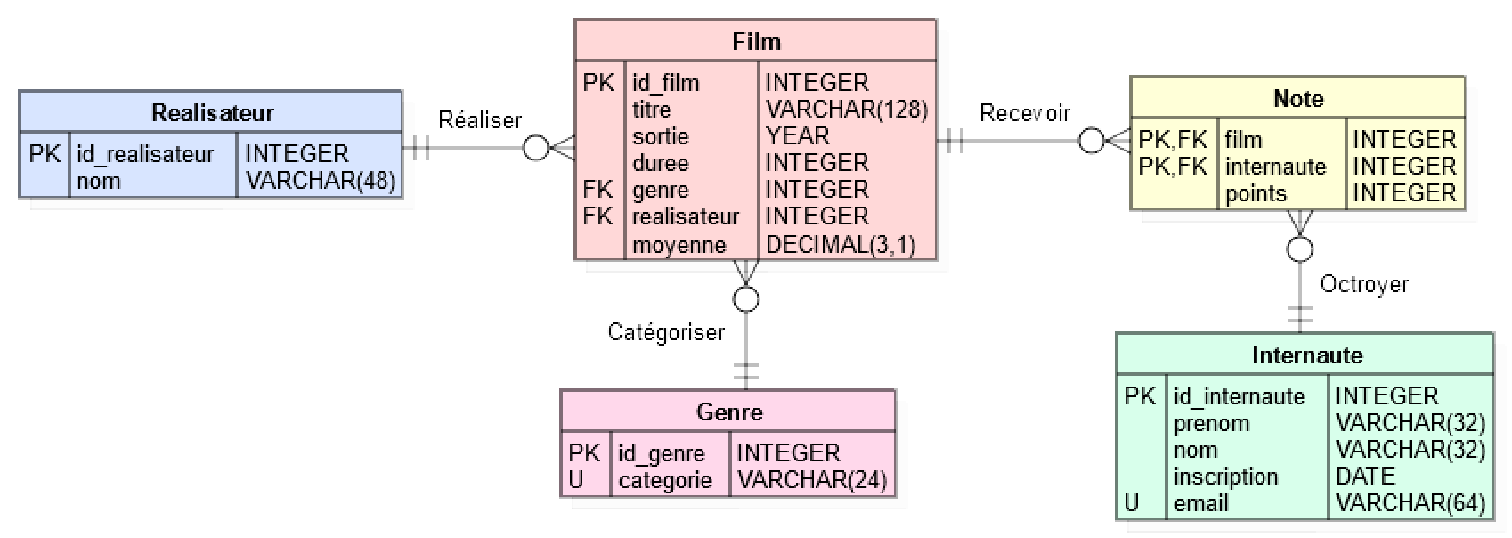
\includegraphics[width=16cm]{img/uml}
\begin{enumerate}[\bfseries 1.]
	\item Que fait la requête \mintinline{sql}{SELECT categorie FROM Genre;} ?

     \begin{encadre}[Réponse]
        Cette requête produit la table de toutes les catégories qui figurent dans la table \textbf{Genre}.
      \end{encadre}

	\item Que fait la requête \mintinline{sql}{SELECT * FROM Realisateur WHERE nom LIKE 'Jean%';} ?

    \begin{encadre}[Réponse]
        Cette requête produit la table des tuples de \texttt{\textbf{Realisateur}} dont le nom commence par Jean.
        \end{encadre}


    \item Que fait la requête suivante ?
            \begin{minted}{sql}
SELECT titre,categorie
FROM Film
    JOIN Genre ON Film(genre) = Genre(id_genre);
            \end{minted}
\begin{encadre}[Réponse]
Cette requête affiche le titre et la catégorie correspondante de tous les films.
\end{encadre}
\item Quelle requête donne la table complète des films sortis en 1984 ?
\begin{sql}
SELECT * FROM Film WHERE sortie = 1984;
\end{sql}

\item Quelle requête donne la table complète des internautes inscrits entre début 2018 et fin 2019 ?
\begin{sql}
SELECT * FROM Internaute
WHERE inscription BETWEEN '2018-01-01' AND '2019-12-31';
\end{sql}


\item Quelle requête donne la table des titres et moyenne des films durant au moins 3h ?
\begin{sql}
SELECT titre,moyenne FROM Film WHERE duree >= 180;
\end{sql}



\item Quelle requête donne la table des titres des films sortis après 2000 et dont la moyenne est supérieure à 8 ?
\begin{sql}
SELECT titre FROM Film WHERE sortie > 2000 AND moyenne >= 8;
\end{sql}

\item  Quelle requête donne la table complète des films d'Alfred Hitchcock ?\\
\begin{sql}
SELECT * FROM Film
    JOIN Realisateur ON Film.realisateur = Realisateur.id_realisateur
WHERE nom = 'Alfred Hitchcock';
\end{sql}

\item  Quelle requête donne la table donnant l'identifiant, le titre et l'année de sortie des thrillers ?

\begin{sql}
SELECT id_film,titre,sortie FROM Film
    JOIN Genre ON genre = id_genre
WHERE categorie = 'thriller';
\end{sql}

\item  Quelle requête donne la table des noms de réalisateurs et titres de films dont la moyenne est 8.5 ou plus ?

\begin{sql}
SELECT nom,titre FROM Realisateur
    JOIN Film ON id_realisateur = realisateur
WHERE moyenne >= 8.5;
\end{sql}

\item  Quelle requête donne la table des prénoms et noms des internautes ayant octroyé 1 seul point à un film,
en supprimant les doublons ?

\begin{sql}
SELECT DISTINCT prenom, nom FROM Internaute
    JOIN Note ON id_internaute = internaute
WHERE points = 1;
\end{sql}

\item Quelle requête donne la table des adresses email et des points des internautes qui ont notés « Les Profs » ?

\begin{sql}
SELECT email,points FROM Internaute
    JOIN Note ON id_internaute = internaute
    JOIN Film ON film = id_film
WHERE titre = 'Les Profs';
\end{sql}

\item La requête suivante échoue. Émettre une hypothèse pour expliquer cet échec.\\
\mintinline{sql}{INSERT INTO Note VALUES(248, 93, 17);}

\begin{encadre}[Réponse]
Le nombre de points attribués n'est pas compris entre 0 et 10.
\end{encadre}

\item Expliquer pourquoi la requête suivante échoue :\\
\mintinline{sql}{DELETE FROM Internaute WHERE id_internaute = 50;}\\

\begin{encadre}[Réponse]
Un enregistrement de la table \textbf{Note} possède une clé étrangère internaute qui se réfère à la clé primaire id\_internaute de valeur 50.
\end{encadre}

\carreauxseyes{16}{4}

\item Donner les requêtes SQL permettant d'inscrire l'utilisateur et le film suivant :\\
Léo Part s'est inscrit sur le site le 21 juin 2020 avec l'adresse mail \texttt{leo.part@alapla.ge}. Il a l'identifiant 104.\\
Il a mis la note de 9 sur 10 au film de science-fiction « Contact » de Robert Zemeckis qui est sorti en 1997 et qui dure 2 h 33 min.\\
Le genre de ce film est 13 et son identifiant 694.\\

\begin{sql}
INSERT INTO Internaute VALUES(104, "Léo", "Part", "2020-06-21", "leo.part@alapla.ge");
INSERT INTO Film VALUES(694, "Contact", 1997, 153, 13, 129, 9.0);
INSERT INTO Note VALUES(694, 104, 9);
\end{sql}

\item Donner les requêtes SQL afin de supprimer le film « Fatal » de la BDD du site CinéHit tout en maintenant son intégrité. L'identifiant du film est 446.

\begin{sql}
DELETE FROM Note WHERE film = 446;
DELETE FROM Film WHERE id_film = 446;
\end{sql}
\end{enumerate}
\end{document}
